Con el \textit{algoritmo de Kruskal} obtenemos un árbol generador de coste mínimo mediante la ordenación de todas las aristas del grafo por su peso (de menor a mayor) y luego añadiendo las que son más baratas (la menores) al árbol de expansión, asegurándose de que no se producen cíclos.

\subsection{Ejemplo algoritmo Kruskal}
Partimos de un grafo ponderado, no dirigido y conexo y guardamos las aristas según su peso.
\begin{figure}[h]
  \begin{center}
    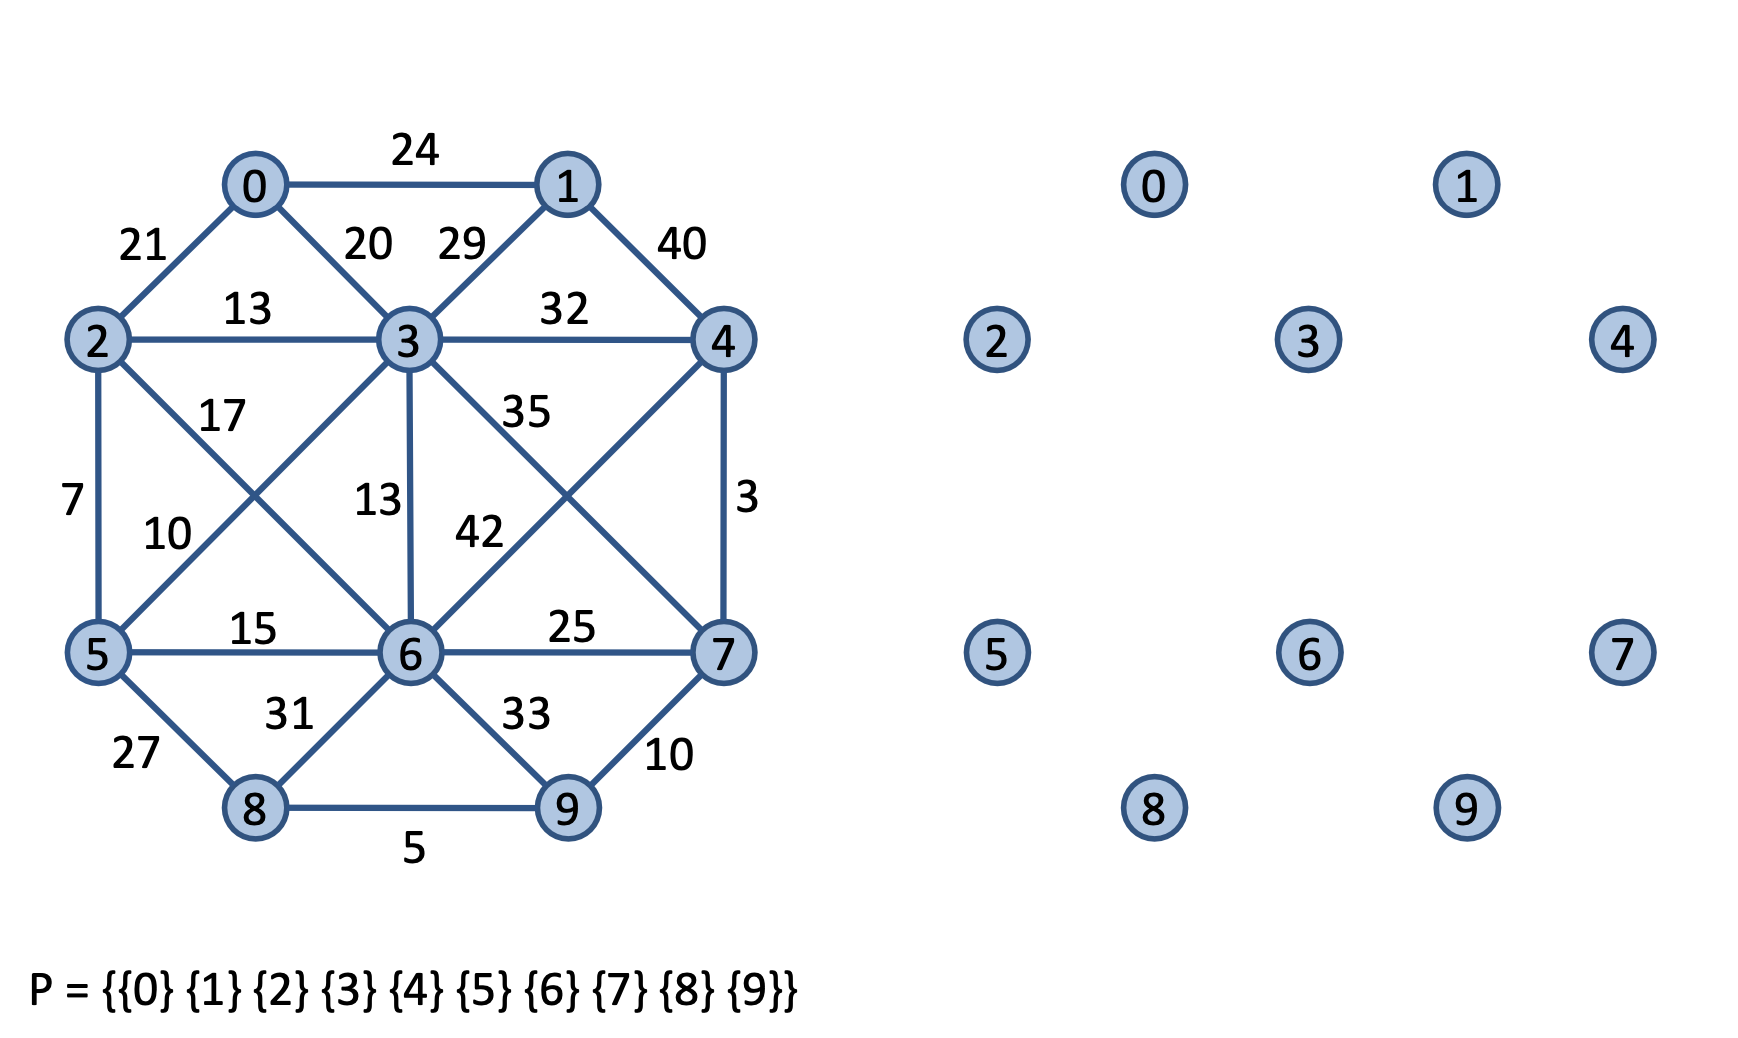
\includegraphics[width=.7\textwidth]{assets/kru1.png}
  \end{center}
  \caption{Ejemplo algoritmo Kruskal}
\end{figure}

Vemos que tenemos el grafo comentado anteriormente, los vértices del mismo pero sin aristas y una partición \(P\) que contiene los subconjuntos a los que pertenece cada elemento (nodo).

Por tanto, para crear obtener el \textit{árbol generador de coste mínimo} cogemos la arista con menor peso y unimos el par de vértices que la contiene, añadiendo en la partición \(P\) los nodos que están unidos en un subconjunto común.

Para ello, vamos a seguir una serie de pasos los cuales como resultado obtendremos el árbol de expansión de coste mínimo:
\begin{enumerate}
  \item Cogemos la arísta con menor coste \(\rightarrow\) \textit{Figura 10.15: Ejemplo 1 Kruskal}.
  \item Unimos los vértices que une dicha arista \(\rightarrow\) realizamos la opración \texttt{unir(P.encontrar(4),\\P.encontrar(7));}, donde buscamos los representantes de cada subconjunto y los unimos (\textit{Figura 10.15.(a)}).
  Si ambos tienen el mismo representante no se unen.
  \item Vemos que los vértices se unen al mismo subconjunto y tienen el mismo representante el cual puede ser el mayor o el menor que unen (\textit{Figura 10.15.(b)}).
  \item Ahora hacemos lo mismo con la siguente arista cuyo valor sea el menor de los valores mayores o igual a la arista anterior (\textit{Figura 10.16.(a)}). 
\end{enumerate}

Para comenzar vamos cogemos la arista cuyo valor sea el más pequeño, este caso será la que une los vértices `4' y `7', con valor 3:
\begin{figure}[h]
  \begin{minipage}{0.4\textwidth}
    \centering
    \begin{subfigure}{\textwidth}
      \centering
      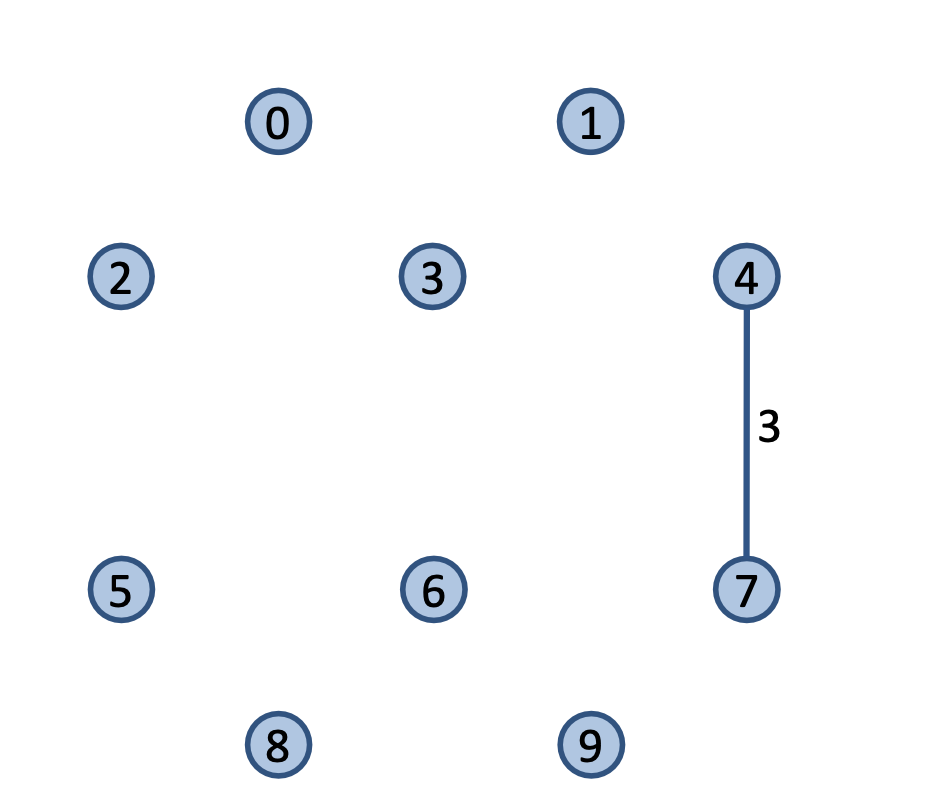
\includegraphics[width=.65\textwidth]{assets/kru2.png}
      \caption{Incluimos la primera arista}
    \end{subfigure}
  \end{minipage}
  \hfill
  \begin{minipage}{0.5\textwidth}
    \centering
    \begin{subfigure}{\textwidth}
      \centering
      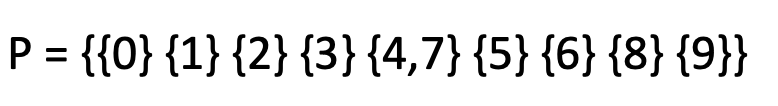
\includegraphics[width=\textwidth]{assets/kru3.png}
      \caption{Incluimos la primera arista que conecta los vértices 4 y 7 y ambos se incluyen en el mismo subconjunto.}
    \end{subfigure}
  \end{minipage}
  \caption{Ejemplo 1 Kruskal}
\end{figure}

Ahora elegimos la siguente arista cuyo valor sea mayor a la de la arista anterior elegida y que no produzca cíclos:
\begin{figure}[h]
  \begin{minipage}{0.4\textwidth}
    \centering
    \begin{subfigure}{\textwidth}
      \centering
      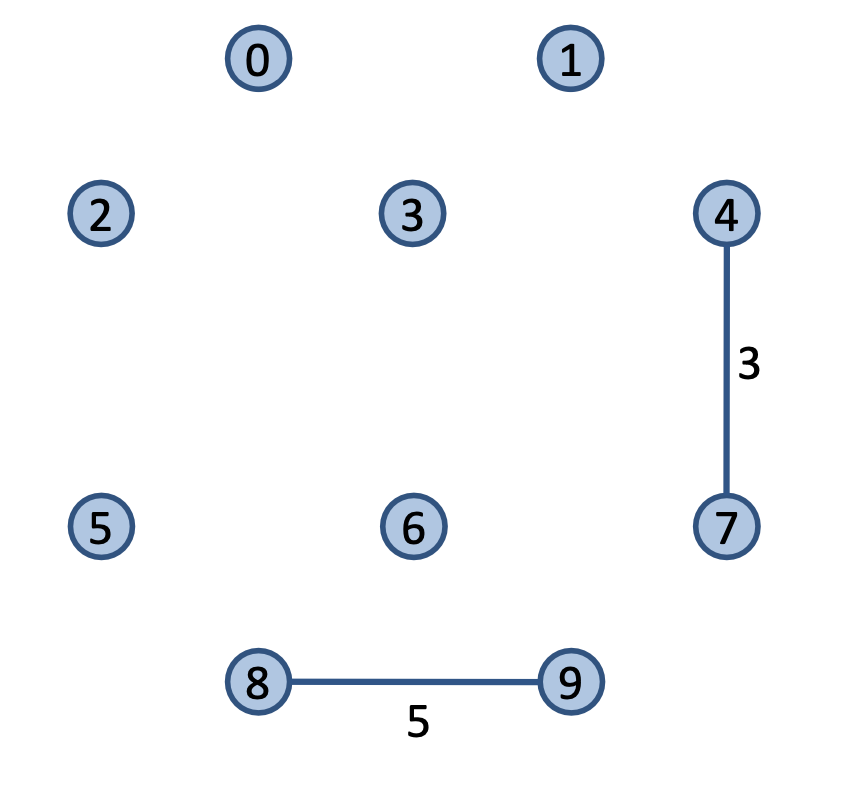
\includegraphics[width=.65\textwidth]{assets/kru5.png}
      \caption{Incluimos la siguente arista con valor \(\geq\) a la anterior}
    \end{subfigure}
  \end{minipage}
  \hfill
  \begin{minipage}{0.5\textwidth}
    \centering
    \begin{subfigure}{\textwidth}
      \centering
      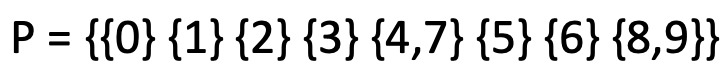
\includegraphics[width=\textwidth]{assets/kru6.png}
      \caption{Se unen los vértices 8 y 9 en el mismo subconjunto}
    \end{subfigure}
  \end{minipage}
  \caption{Ejemplo 2 Kruskal}
\end{figure}

Hacemos esto hasta que tengamos todos los nodos unidos sin ciclos, muy importante debido a que en los árboles no hay ciclos, y como resultado tenemos:

\begin{figure}[h]
  \begin{center}
    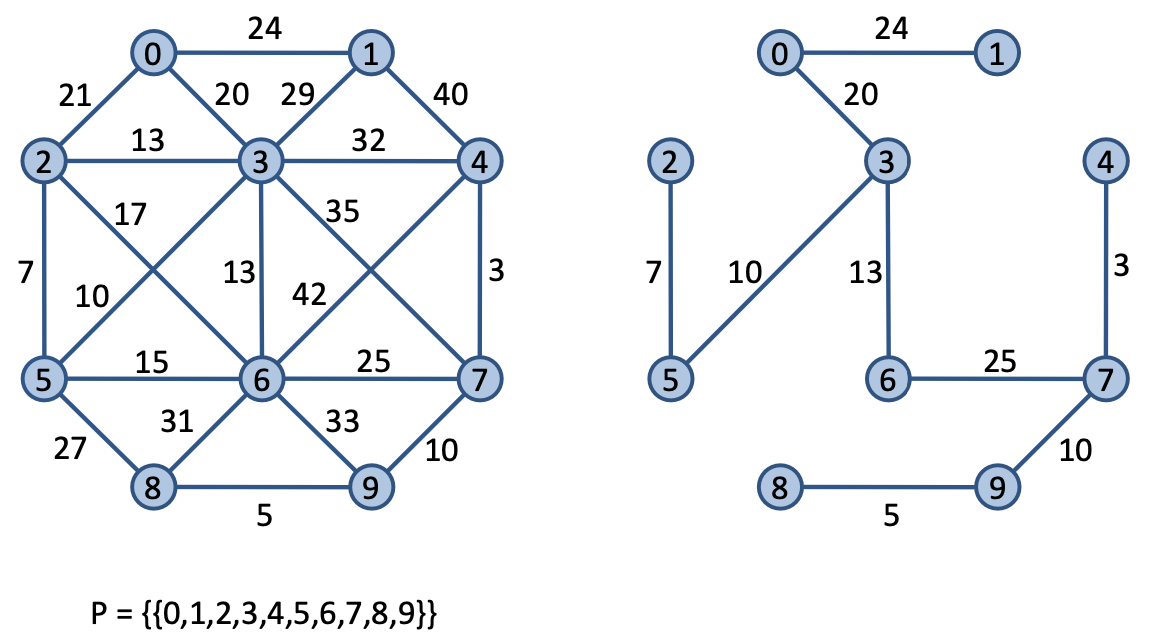
\includegraphics[width=.7\textwidth]{assets/kru4.png}
  \end{center}
  \caption{Resultado ejemplo algoritmo Kruskal}
\end{figure}

Como hemos conseguido una partición que contiene un único subconjunto de vértices, no nos hace falta recorrer más la lista de las aristas ni el grafo debido a que todos los vértices están unidos mediante las aristas con los costes mínimos, en definitiva tenemos termiando el \textit{árbol de expansión de coste mínimo}.


